\section{Generalized Distributed Resource Management Architecture}

Traditional distributed computing platforms can be split into two layers, the
control plane and the data plane.

\begin{figure}[ht]
  \centering
  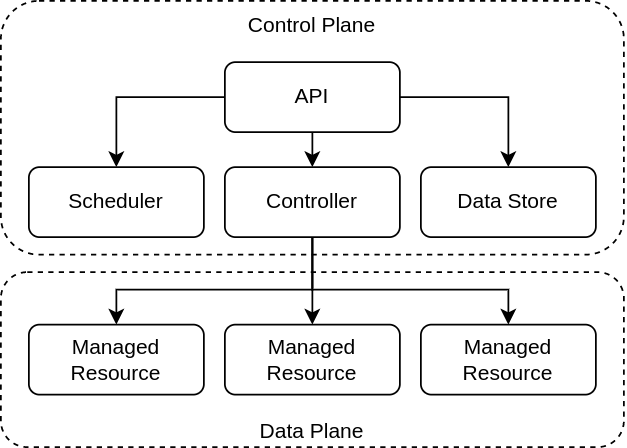
\includegraphics[width=0.6\linewidth]{resources/dynamic-distributed-resource-management-overview.png}
  \caption{Overview over general components in a Dynamic Distributed Resource Management System}
  \label{fig:ddrms-overview}
\end{figure}

The control plane is a set of components that make global decisions about the
distributed system as a whole and acts as a single source of truth regarding the
configuration and state of all components and resources in the distributed
system.

The control plane generally consists of the following components:

\begin{description}
  \item[Data Store]
    Responsible for consistently storing the current configuration and state of
    all components and resources.
  \item[API]
    An interface for users, administrators, and other components in the
    distributed system to interact with.
  \item[Controller(s)]
    A component or set of components responsible for managing all or a specific
    type of computing resources.
  \item[Scheduler]
    Component responsible with determining the physical location of a newly
    requested computing resource.
\end{description}

The data plane aggregates the computing resources managed by the control plane,
for instance virtual or physical machines, storage, networks, or more abstract
resources like services, tasks, or secrets.

Customers usually interact with the system by using for example graphical or
terminal applications. There are no additional services that are expected to be
managed by the customer.

\section{Thread Vectors}

Infrastructure
\begin{itemize}
  \item Memory (in-scope)
  \item Physical (out-of-scope)
\end{itemize}

Platform
\begin{itemize}
  \item Arbitrary code execution (in-scope)
  \item Code modification (in-scope)
  \item Supply-chain (in-scope)
\end{itemize}

Software threads out-of-scope

\subsection{IaaS Service Model}

In the IaaS Service Model the infrastructure provider would offer the capability
of allocating infrastructure to the application owner and the application owner
would be responsible for deploying and orchestrating application workloads onto
said infrastructure.

\begin{figure}[ht]
  \centering
  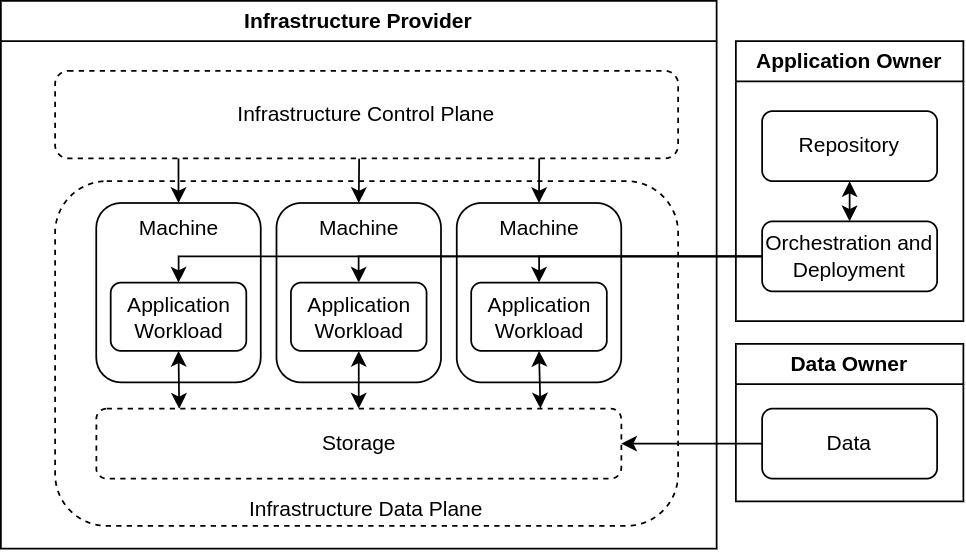
\includegraphics[width=0.8\linewidth]{resources/distributed-computing-infrastructure-architecture.png}
  \caption{IaaS service model architecture overview.}
  \label{fig:iaas-model-architecture}
\end{figure}

Even though the application owner manages and controls the software stack
running on the executed infrastructure, the infrastructure provider is still
able to read and manipulate the main memory of the provided machines.

\subsection{PaaS Service Model}

As outlined in the confidential computing section techniques for shielding data
at rest and in transit are commonly used. For this reason we will simplify the
architecture view by leaving out the storage and network infrastructure.
Applying the generalized distributed resource management architecture to a PaaS
service model, we now get the following architecture:

\begin{figure}[ht]
  \centering
  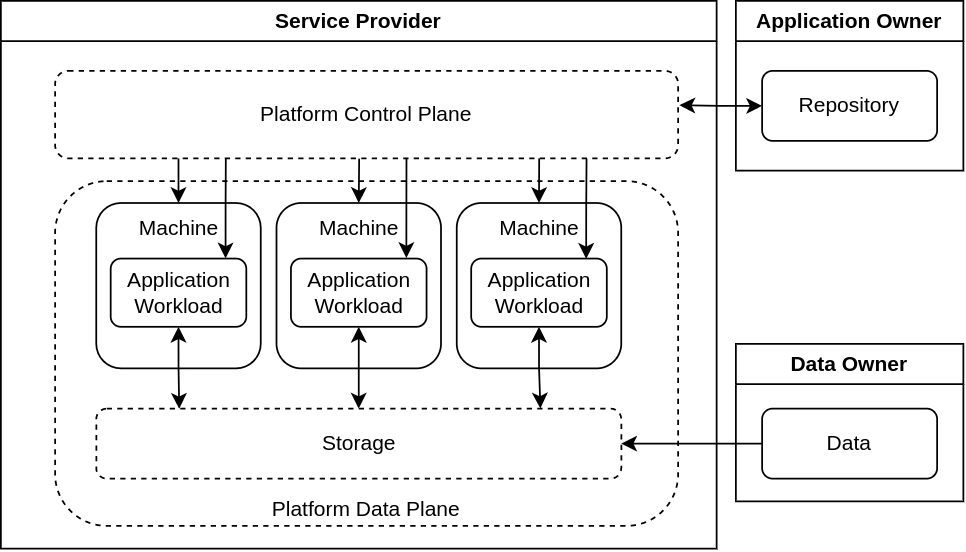
\includegraphics[width=0.8\linewidth]{resources/distributed-computing-platform-architecture.png}
  \caption{Distributed computing platform architecture overview.}
  \label{fig:distributed-computing-platform-architecture}
\end{figure}

The illustrated control plane in figure
\ref{fig:distributed-computing-platform-architecture} is a combination of the
infrastructure and platform control plane. While the infrastructure control
plane allocates infrastructure, the platform control plane deploys and
orchestrates application workloads on said infrastructure. In order to do so the
platform control plane create execution environments for application workloads
and executes application code provided by the application owner through a
repository. This implies that the platform control plane is able to execute
arbitrary code inside the execution environments it created. And because the
service provider manages the control plane, the data owner has to trust the
service provider to run only unmodified application code on his/her data.

The data owner could try to use encryption techniques in order to shield the
data from the service provider and only provide the decryption key to running
application workloads after verifying their integrity, but because the service
provider is able to execute arbitrary code in the provided execution
environments, it would still be to modify the running workload after the
decryption key has been supplied.

\subsection{SaaS Service Model}

\todo[inline]{Service Provider would become application owner, defeats purpose}
